\chapter{Model trajectories directly using a Gaussian Process}\label{chap:direct_gp}
 A tempting solution is to directly apply the \acrshort{gp} framework introduced in \cref{chap:theory} and model the vessel's trajectory as a function of time $\vec{f}(\tau)$. However, as there are no observations of the target vessel's future position, there is no actual data to condition the \acrshort{gp} on. Instead, this chapter will attempt to use nearby trajectories and assume these historical trajectories to resemble the future trajectory of the target vessel. 

\section{Method}
While a pure function of time is tempting, it is unable to differentiate between different historical trajectories. To utilize as much of the available information in a single \acrshort{ais} message as possible, and in order to compensate for any initial differences in position, velocity or course of nearby trajectories, a bit more complex formulation $\vec{f}(\boldsymbol{x}_0, \psi_0, v_0, \tau): \mathcal{R}^5 \to \mathcal{R}^2$ is proposed. The key variables are explained in \cref{table:posgp_key_variables}.

\begin{table}[h]
    \centering
    \begin{tabular}{ll}
        \textit{\textbf{Variable}}              & \textit{\textbf{Description}}      \\ \hline
        $\boldsymbol{x}_0 \in \mathcal{R}^2$    & Trajectory's initial position       \\
        $\mathcal{X}_0 \in [0, 360)$            & Trajectory's initial \acrshort{cog} \\
        $v_0 \in \mathcal{R}$                   & Trajectory's initial \acrshort{sog} \\
        $\tau \in [0, \infty)$                  & Prediction timestamp               \\
        $\boldsymbol{x}_\tau \in \mathcal{R}^2$ & Predicted position                 \\
    \end{tabular}
    \caption{Key variables}
    \label{table:posgp_key_variables}
\end{table}
The method is formulated in mathematical terms in \cref{eq:gp_direct}. This will from now on be referred to as the \textit{Direct \acrshort{gp}} approach, as it directly utilizes a \acrshort{gp} to predict the trajectory.

\begin{subequations}\label{eq:gp_direct}
    \begin{align}
        \boldsymbol{f}(\boldsymbol{\eta}) & = \boldsymbol{x}_{\tau} \label{eq:gp_direct_f}, \quad \boldsymbol{\eta} = \begin{bmatrix} \boldsymbol{x}_0 & \psi_0 & v_0 & \tau\end{bmatrix}                   \\
        \boldsymbol{f}(\boldsymbol{\eta}) & \sim \text{GP}(\boldsymbol{m}(\boldsymbol{\eta}), K(\boldsymbol{\eta}, \boldsymbol{\eta}))\label{eq:gp_direct_f_dist}
    \end{align}
\end{subequations}

The function $\vec{f}$ can be conditioned on similar trajectories using \cref{alg:gp_prediction} from \cref{chap:theory}, and then be used to answer queries about the likely trajectories that the vessel might follow. An example output is available in \cref{fig:direct_gp_example}.

\subsection{Key Assumption}
This formulation builds on the key assumption that the target vessel is following the same underlying trajectory as the nearby historical trajectories. In other words, the function $\vec{f}$ does not represent the target vessel's future trajectory; it merely interpolates the past trajectories with similar initial conditions. 


%The conceptual benefits of this formulation includes:
%\begin{description}
%    \item[Continuous formulation] The model directly models the position at any time $\tau$ and does not require discretization. It can therefore be queried for any continuous timestamp $\tau$.
%    \item[Conceptually easy] This formulation directly expresses the unknown trajectory, making it conceptually simple to understand.
%    \item[Simple Problem formulation] The model requires few components and builds directly on the \acrshort{gp}s introduced in \cref{chap:theory}.
%    \item[Easy incorporation of available AIS data] The reported \acrshort{cog} and \acrshort{sog} can easily be incorporated into the similarity measure, utilizing more of the available data.
%\end{description}

\subsection{Choice of Kernel}
Many different kernels may work well with this formulation. This section will cover a few alternatives that works well in practice, but there are likely many other alternatives that may work just as well, if not better. 

The \acrshort{rbf} kernel was found to work well with the formulation used in this chapter. Along the traffic lanes, vessels tend to move in a smooth trajectory, which makes the \acrshort{rbf} kernel a good choice. As the function arguments are of different scales, it is a good idea to use different lengthscales for each input dimension, i.e.

\begin{equation}
    k(\boldsymbol{\eta}, \boldsymbol{\eta}') = \sigma^2 \exp \big[ (\boldsymbol{\eta} - \boldsymbol{\eta}') W^{-1} (\boldsymbol{\eta} - \boldsymbol{\eta})^\intercal \big]
\end{equation}
where $W$ is a diagonal matrix with a separate lengthscale for each dimension and $\sigma^2$ is a scale parameter. This kernel yields smooth functions for $\vec{f}$ and is well suited to model the general trend of the trajectory.

In some scenarios, a single \acrshort{rbf} kernel results in an unreasonably smooth function. Adding a second \acrshort{rbf} kernel as in \cref{eq:direct_gp_kernel} works well in these scenarios, as it gives the model some additional flexibility in local regions. However, it makes hyperparameter selection significantly more complicated as the optimal solution is no longer unique.  

\begin{equation}\label{eq:direct_gp_kernel}
    k(\boldsymbol{\eta}_i, \boldsymbol{\eta}_j) = \sigma_0 k_0(\boldsymbol{\eta}_i, \boldsymbol{\eta}_j) + \sigma_1 k_1(\boldsymbol{\eta}_i, \boldsymbol{\eta}_j)
\end{equation}

Each term in this kernel offers a unique interpretation:
\begin{description}
    \item[Long term trend $k_0$] is an \acrshort{rbf} kernel intended to cover the long-term behavior of the trajectories, i.e., a smooth component describing the overall trend of the trajectories. The length scales of this kernel are expected to be relatively large.
    \item[Dependent noise $k_1$] is an \acrshort{rbf} kernel intended to model the local variations between different trajectories which is not well explained by $k_0$. The length scales are therefore expected to be short.
\end{description}

\section{Implementation Details}

This formulation builds directly on the \acrshort{gp} framework introduced in \cref{chap:theory} and the trajectory can be conditioned on available training data using \cref{alg:gp_prediction}. 

\subsection{Approximate Gaussian Process}
Another promising approach is to utilize an approximation technique to avoid the scalability issue of \acrshort{gp}s. While this thesis focuses on specific scenarios, as discussed in \cref{chap:ais}, the formulation in this chapter lends itself nicely to using more data. Though not implemented in this thesis, the \acrshort{svgp} introduced in \cref{chap:theory} is one such method that attempts to fit a \acrshort{gp} while simultaneously finding a good subset of the data to summarize the full dataset.


\begin{figure}
    \centering
    \begin{subfigure}{\textwidth}
        \centering
        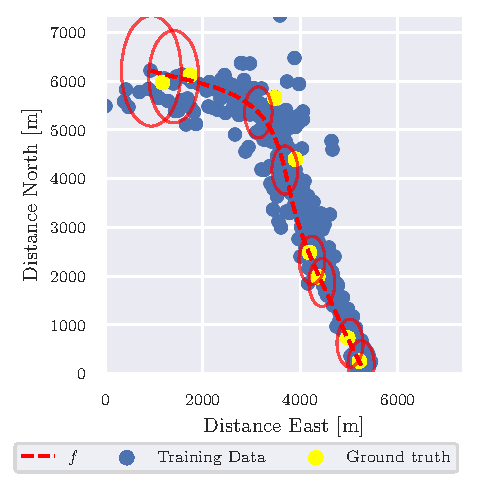
\includegraphics{figures/direct_gp_example.pdf}
        \caption{The predicted trajectory using the direct \acrshort{gp} formulation. The ellipses are the $95\%$ CI for the prediction at the ground truth timestamps.}
    \end{subfigure}
        \begin{subfigure}{\textwidth}
        \centering
        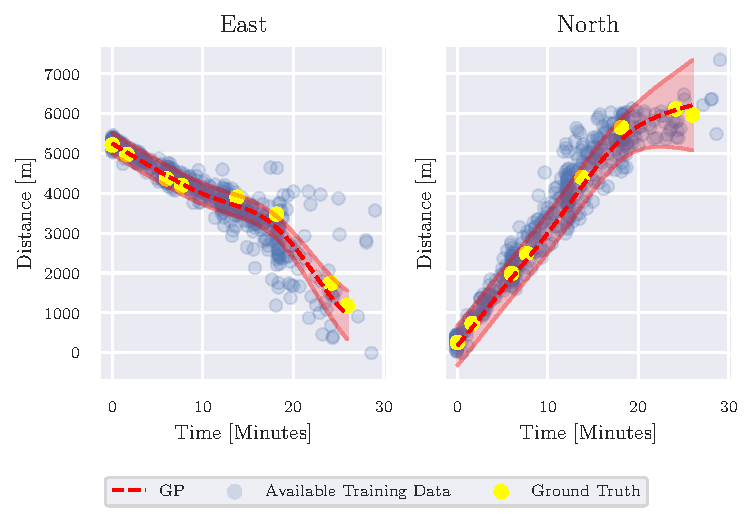
\includegraphics{figures/direct_gp_state_example.pdf}
        \caption{The East and North components plotted against time with a $95\%$ CI.}
    \end{subfigure}
    \caption{Example output from the Direct \acrshort{gp} approach. }
    \label{fig:direct_gp_example}
\end{figure}